\documentclass{beamer}
\usepackage[utf8]{inputenc}
\usepackage[french]{babel}
\usepackage{xmpmulti}
\usepackage{amsmath}
\usepackage{amsfonts}
\usepackage{amssymb}
\usepackage{wasysym}
\usetheme{Warsaw}
\usecolortheme{beaver}
\setbeamertemplate{navigation symbols}{}
\usepackage{tikz}
\usetikzlibrary{calc}

\definecolor{pbblue}{HTML}{0A75A8}% color for the progress bar and the circle

\makeatletter
\def\progressbar@progressbar{} % the progress bar
\newcount\progressbar@tmpcounta% auxiliary counter
\newcount\progressbar@tmpcountb% auxiliary counter
\newdimen\progressbar@pbht %progressbar height
\newdimen\progressbar@pbwd %progressbar width
\newdimen\progressbar@rcircle % radius for the circle
\newdimen\progressbar@tmpdim % auxiliary dimension

\progressbar@pbwd=\linewidth
\progressbar@pbht=1pt
\progressbar@rcircle=2.5pt

% the progress bar
\def\progressbar@progressbar{%

    \progressbar@tmpcounta=\insertframenumber
    \progressbar@tmpcountb=\inserttotalframenumber
    \progressbar@tmpdim=\progressbar@pbwd
    \multiply\progressbar@tmpdim by \progressbar@tmpcounta
    \divide\progressbar@tmpdim by \progressbar@tmpcountb

  \begin{tikzpicture}
    \draw[pbblue!30,line width=\progressbar@pbht]
      (0pt, 0pt) -- ++ (\progressbar@pbwd,0pt);

    \filldraw[pbblue!30] %
      (\the\dimexpr\progressbar@tmpdim-\progressbar@rcircle\relax, .5\progressbar@pbht) circle (\progressbar@rcircle);

    \node[draw=pbblue!30,text width=3.5em,align=center,inner sep=1pt,
      text=pbblue!70,anchor=east] at (0,0) {\insertframenumber/\inserttotalframenumber};
  \end{tikzpicture}%
}

\setbeamertemplate{footline}
{%
  \begin{beamercolorbox}[wd=\paperwidth,ht=4ex,center,dp=1ex]{white}%
    \progressbar@progressbar%
  \end{beamercolorbox}%
}


\setbeamertemplate{headline}{}
\newcommand{\argmin}{\operatornamewithlimits{argmin}} 

\title[P300 BCI without training]{OpenplacOS : Automate your DIY system}
\author[A. Barachant, V. Lagorsse]{Vincent Lagorsse, Alexandre Barachant}\institute{}
\date{RMLL 2013}
\makeatother

\AtBeginSection[]{
{
\setbeamertemplate{footline}{} 
   \begin{frame}{Plan}
   %%% affiche en début de chaque section, les noms de sections et
   %%% noms de sous-sections de la section en cours.
   \tableofcontents[currentsection,hideothersubsections]
   \end{frame} 
   }
\addtocounter{framenumber}{-1}
}
	

\begin{document}

{
\setbeamertemplate{footline}{} 
\begin{frame}
  \titlepage
\end{frame}
}
\addtocounter{framenumber}{-1}

\section{Introduction}

\begin{frame}{Introduction}
\begin{block}{OpenplacOS}
Automation for DIY systems
\end{block}
\end{frame}

\begin{frame}{Examples}
\begin{columns}
\begin{column}[l]{0.5\textwidth}
\begin{figure}
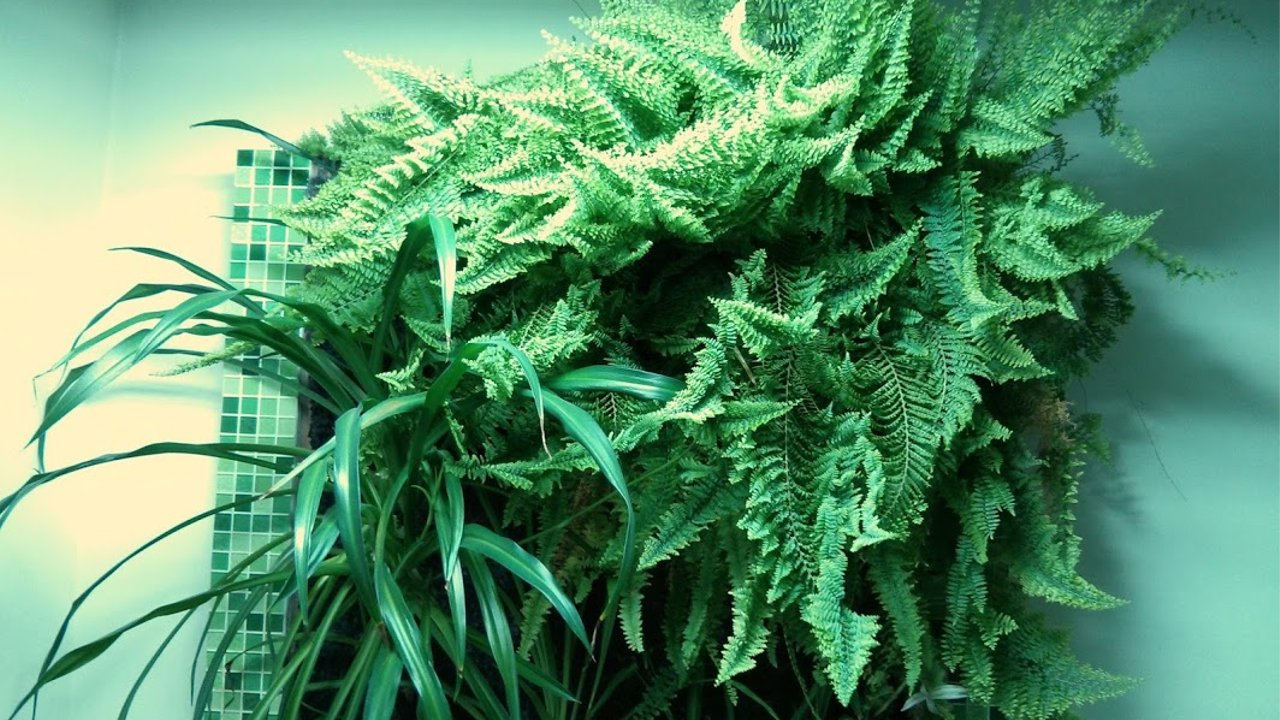
\includegraphics[width=\columnwidth]{figures/mur.jpg}
\end{figure}
\vfill
\textbf{Aquariums, Indoor garden :}
\begin{itemize}
\item Lights
\item Pumps
\item Watering
\item Nutriement, pH
\item Temperature, $\mathrm{CO}_2$
\end{itemize}
\end{column}
\begin{column}[r]{0.5\textwidth}
\textbf{DIY Brewery :}
\begin{itemize}
\item Temperature
\item Process control
\end{itemize}
\vfill
\begin{figure}
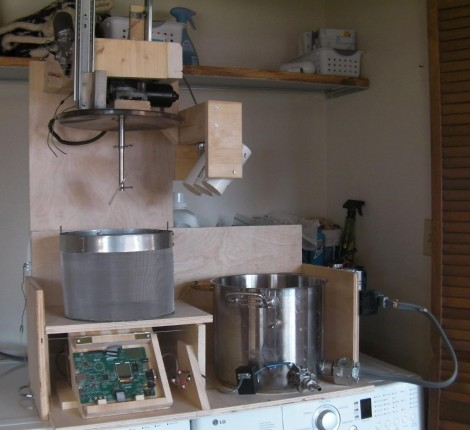
\includegraphics[width=0.8\columnwidth]{figures/brewery.jpg}
\end{figure}
\end{column}
\end{columns}
\end{frame}

\begin{frame}{Hardware Solutions}
\begin{columns}
\begin{column}[l]{0.5\textwidth}
\textbf{Commercial products :}
\begin{itemize}
\item[\Large\smiley] Ready to use
\item[\Large\frownie] Expensive
\item[\Large\frownie] Closed \& No Fun !

\end{itemize}
\end{column}
\begin{column}[r]{0.5\textwidth}
\begin{figure}
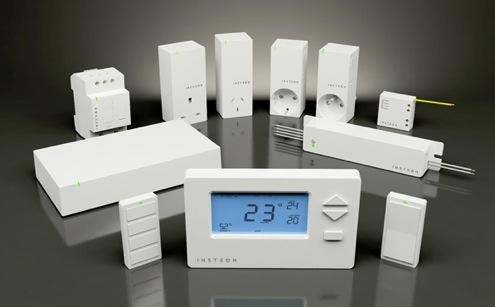
\includegraphics[width=\columnwidth]{figures/Home-Automation-Products.jpg}
\end{figure}
\end{column}
\end{columns}

\begin{columns}
\begin{column}[l]{0.5\textwidth}
\textbf{DIY / Open Hardware :}
\begin{itemize}
\item[\Large\smiley]Flexible
\item[\Large\smiley]Fun but Time Consuming
\item[\Large\frownie] Require electronic and programming skills
\end{itemize}
\end{column}
\begin{column}[r]{0.5\textwidth}
\begin{figure}
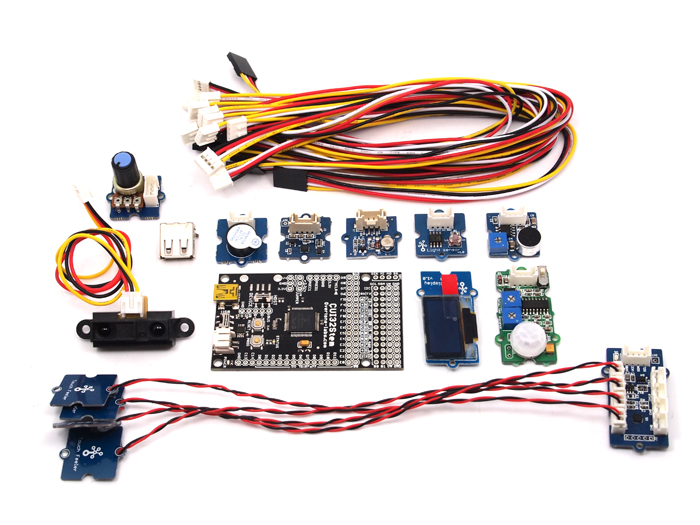
\includegraphics[width=\columnwidth]{figures/kit.jpg}
\end{figure}
\end{column}
\end{columns}
\end{frame}

\begin{frame}{Software Solutions}
\begin{columns}
\begin{column}[l]{0.5\textwidth}
\textbf{Home Automation software :}
\begin{itemize}
\item[\Large\smiley] User friendly
\item[\Large\frownie] Application specific

\end{itemize}
\end{column}
\begin{column}[r]{0.5\textwidth}
\begin{figure}
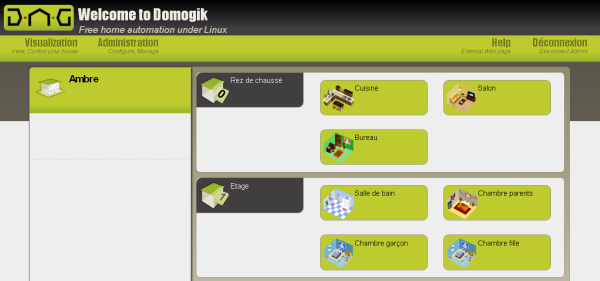
\includegraphics[width=\columnwidth]{figures/screen_domogik.png}
\end{figure}
\end{column}
\end{columns}

\begin{columns}
\begin{column}[l]{0.5\textwidth}
\textbf{Embed software Framework  :}
\begin{itemize}
\item[\Large\smiley] Customizable

\item[\Large\frownie] Hardware specific
\item[\Large\frownie] Low level

\end{itemize}
\end{column}
\begin{column}[r]{0.5\textwidth}
\begin{figure}
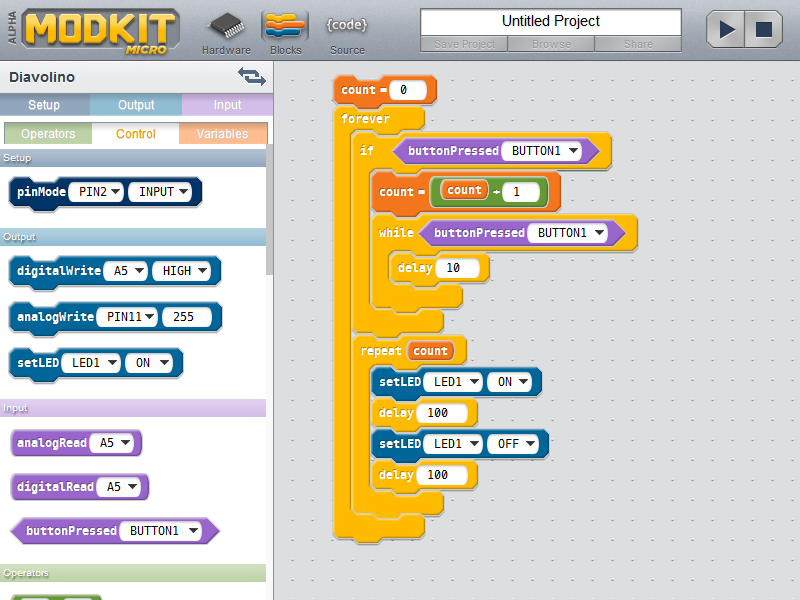
\includegraphics[width=0.9\columnwidth]{figures/modkit.png}
\end{figure}
\end{column}
\end{columns}
\end{frame}

\begin{frame}{OpenplacOS}
\begin{block}{OpenplacOS : }
Flexibility of Open Hardware with the power of home Automation.
\begin{itemize}
\item[\Large\smiley] Usability of an high level home automation software
\item[\Large\smiley] Application agnostic 
\item[\Large\smiley] Customizability
\item[\Large\smiley] Fun !
\end{itemize}
\end{block}
\end{frame}

\section{Principles}
\begin{frame}{Hardware}
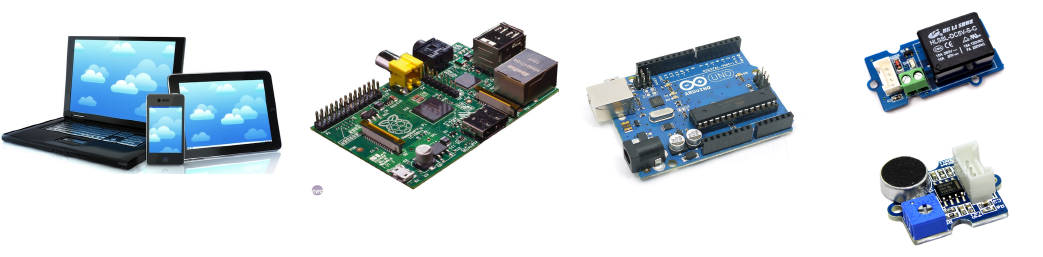
\includegraphics[width=1\columnwidth]{figures/hardware.png}


\begin{columns}
\begin{column}[l]{0.25\textwidth}
\begin{center}User devices\end{center}
\end{column}
\begin{column}[l]{0.25\textwidth}
\begin{center}Host (raspi)\end{center}
\end{column}
\begin{column}[r]{0.25\textwidth}
\begin{center}arduino\end{center}
\end{column}
\begin{column}[r]{0.25\textwidth}
\begin{center}sensors\end{center}
\end{column}
\end{columns}
\end{frame}

\begin{frame}{Hardware Abstraction}
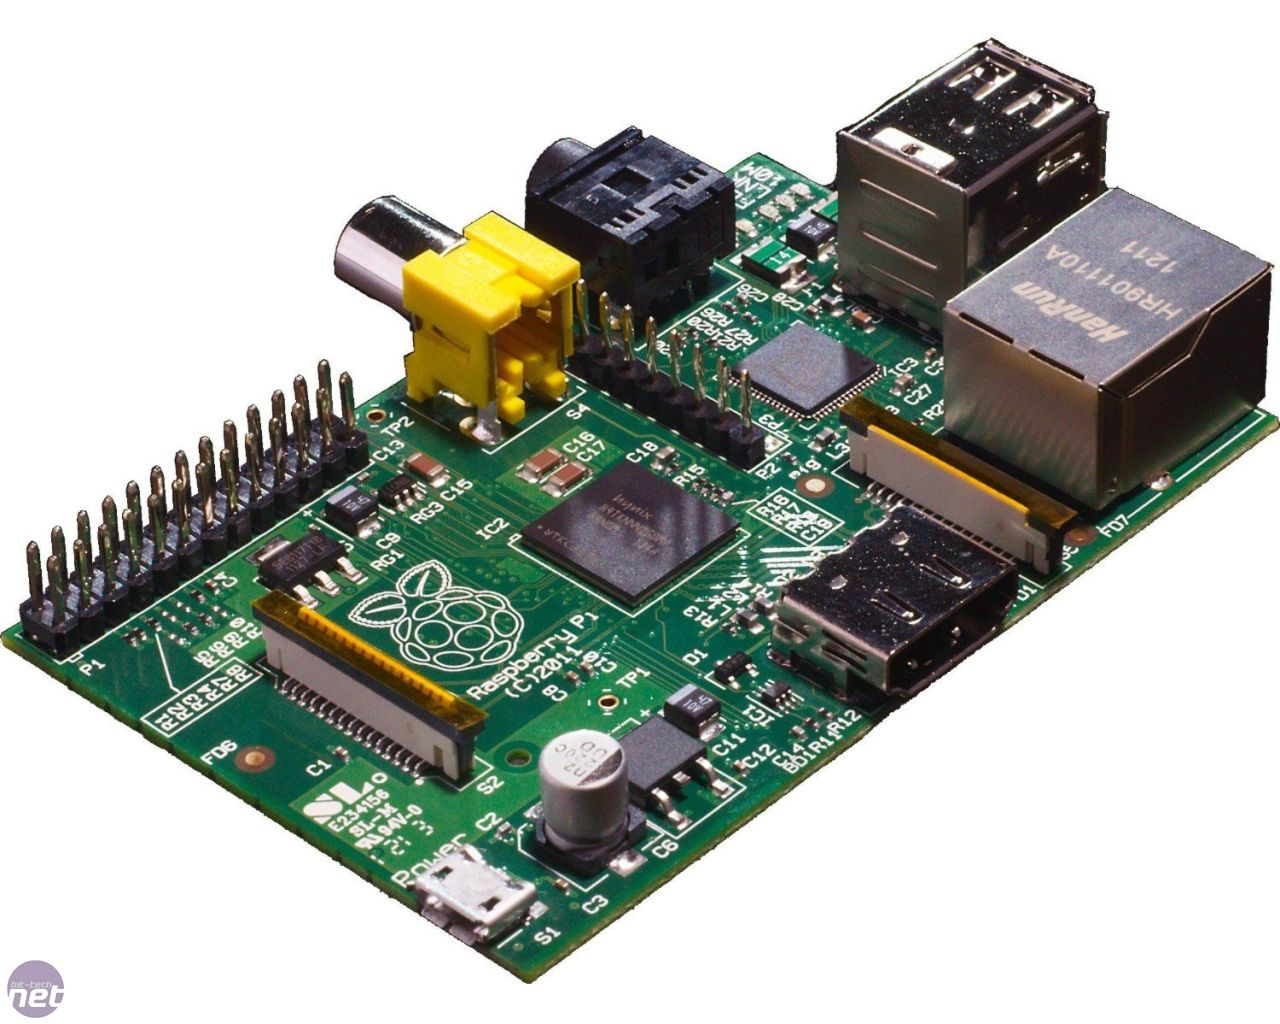
\includegraphics[width=0.12\columnwidth]{figures/raspi.jpg}
\begin{columns}
\begin{column}[l]{0.5\textwidth}
Openplacos \\
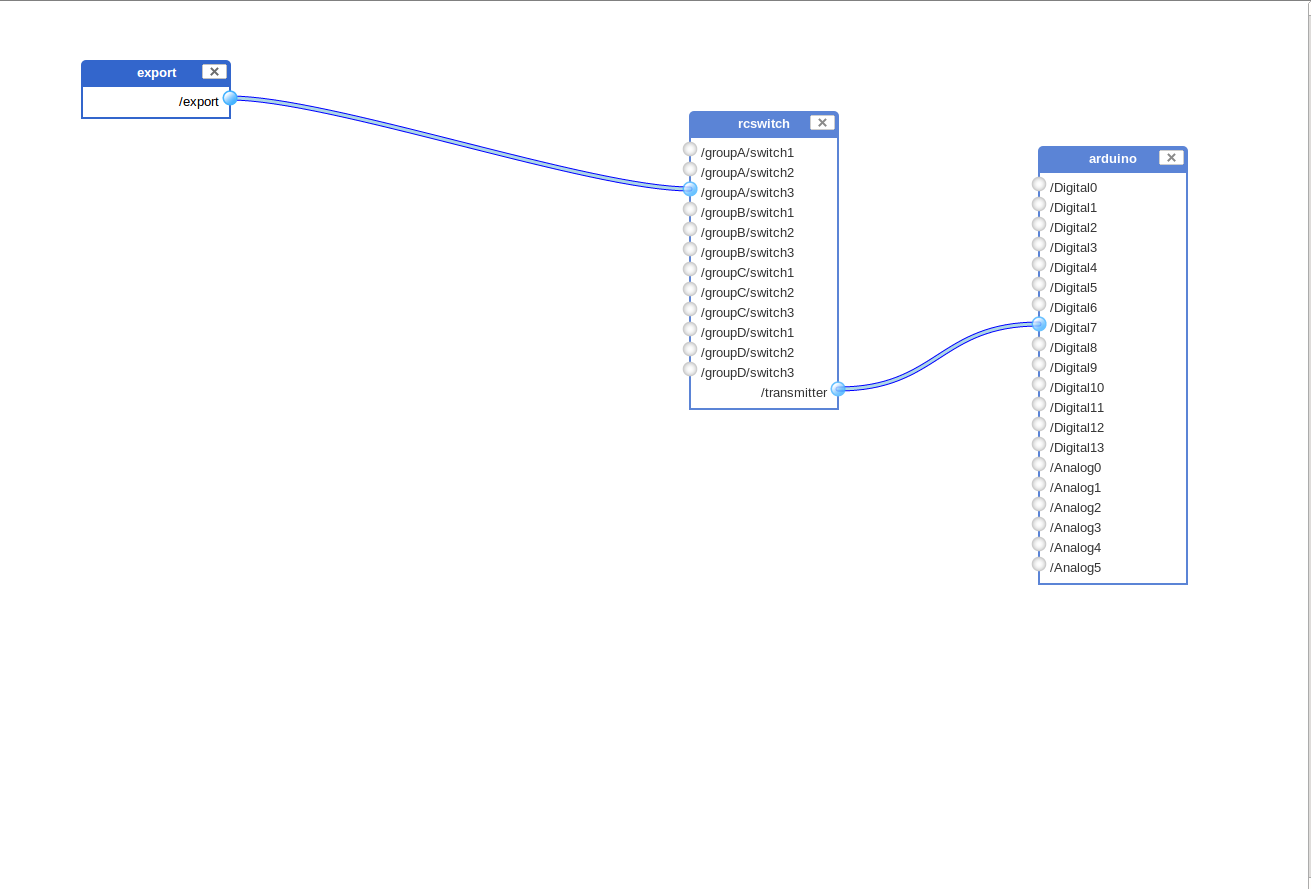
\includegraphics[width=0.9\columnwidth]{figures/config1.png}
\end{column}
\begin{column}[r]{0.5\textwidth}
Real World
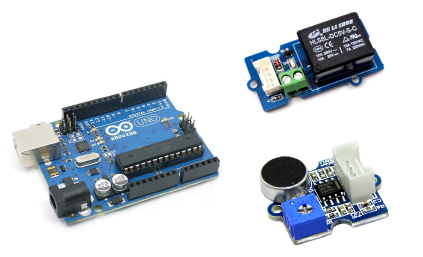
\includegraphics[width=\columnwidth]{figures/HWworld.png}
\end{column}
\end{columns}
\end{frame}

\begin{frame}{FrontEnd}
\begin{columns}
\begin{column}[l]{0.5\textwidth}
Interface
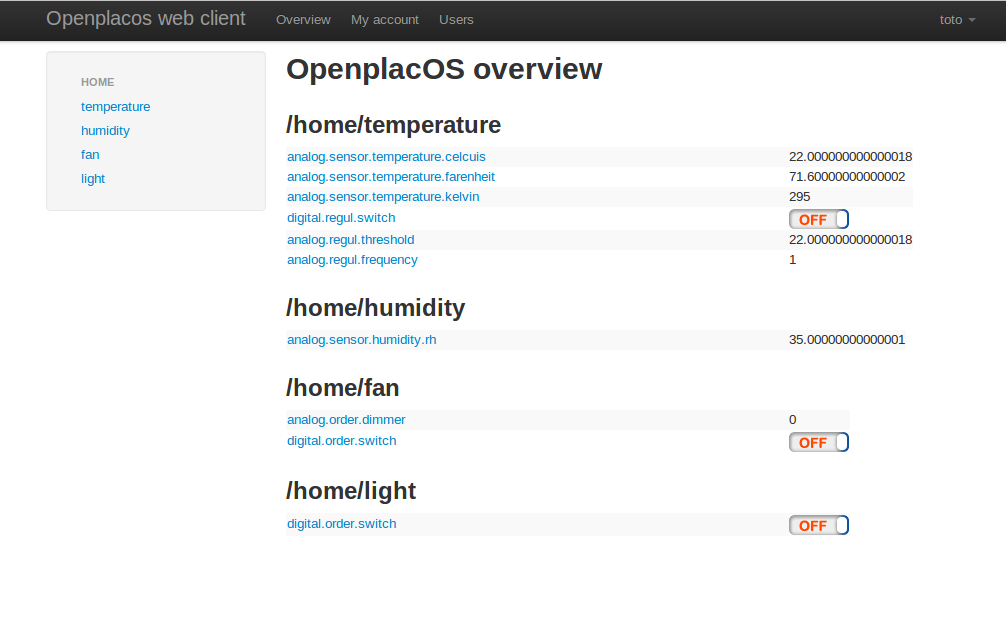
\includegraphics[width=\columnwidth]{figures/opos-overview.png}
\end{column}
\begin{column}[r]{0.5\textwidth}
Openplacos \\
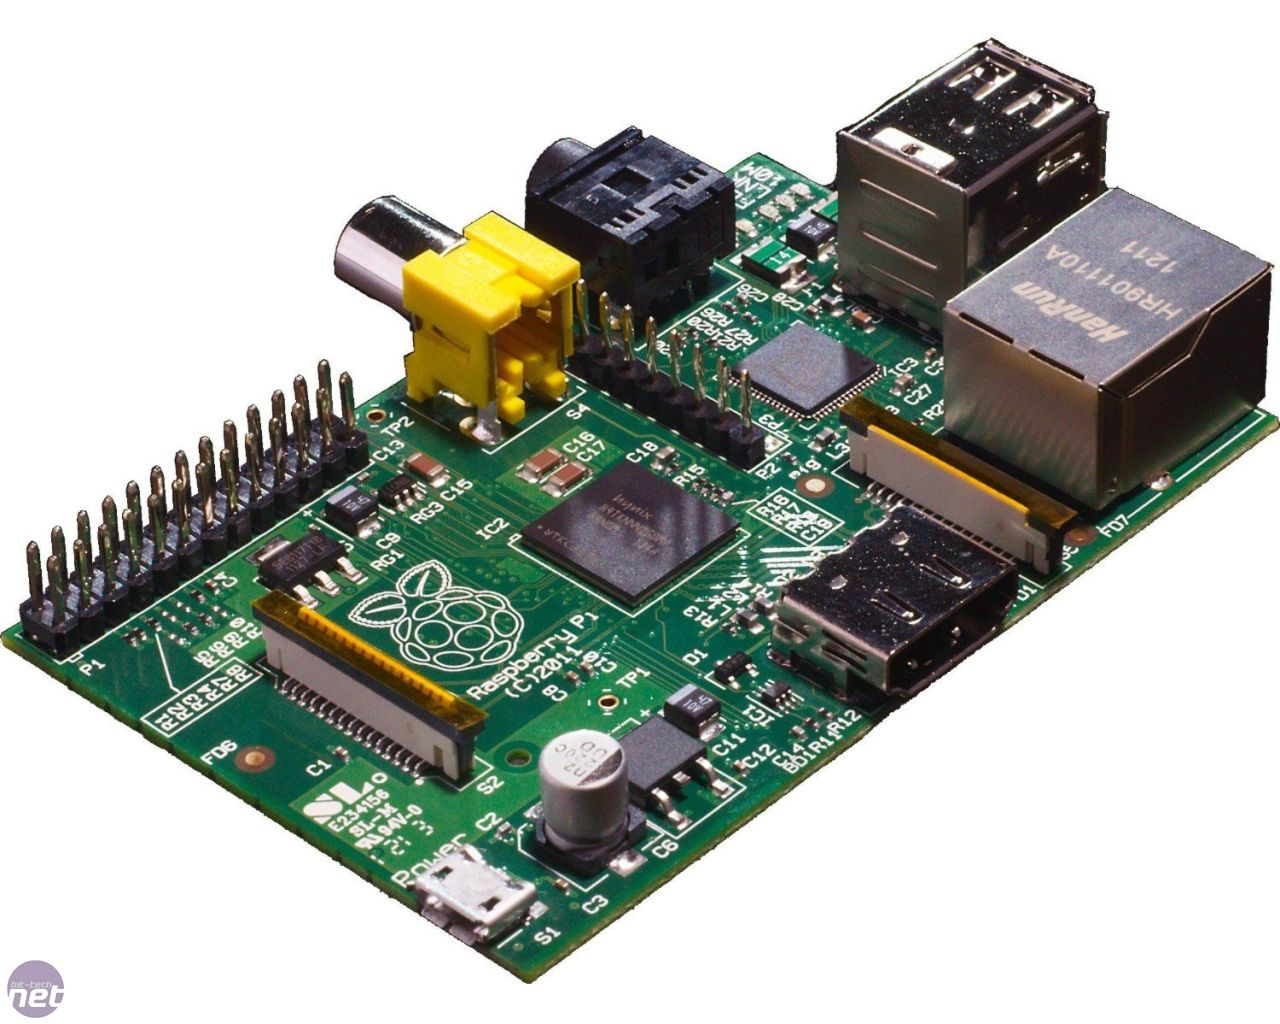
\includegraphics[width=0.3\columnwidth]{figures/raspi.jpg}
\end{column}
\end{columns}
\end{frame}

\section{Software Architecture}

\begin{frame}{Software architecture}
\textbf{3 kind of programs:}
\begin{enumerate}
\item Components
\begin{itemize}
\item[$\Rightarrow$] Abstract Hardware (Arduino, Sensors)
\item[$\Rightarrow$] Process control (PID controller, Automation)
\end{itemize}
\item Clients
\begin{itemize}
\item[$\Rightarrow$] User Interfaces (Web, CLI)
\end{itemize}
\item Core Server
\begin{itemize}
\item[$\Rightarrow$] Component glue
\item[$\Rightarrow$] API for clients
\end{itemize}

\end{enumerate}


\end{frame}

\begin{frame}{Components}
A component is a program which has a specific target. It has inputs and outputs. For example:
\begin{itemize}
\item[$\Rightarrow$] Temperature component: convert raw analog value to celcius
\item[$\Rightarrow$] PID controler: control an actuator according to a consign
\item[$\Rightarrow$] RF relay: manage RF remote switch protocol and mapping
\end{itemize}

\end{frame}
\begin{frame}{Components}
Component inputs and outputs are bind with OpenplacOS server using D-Bus. 
 \begin{itemize}
\item[$\Rightarrow$] Can be written in any langage
\item[$\Rightarrow$] Can run standalone (easy debug)
\end{itemize}
\begin{center} 
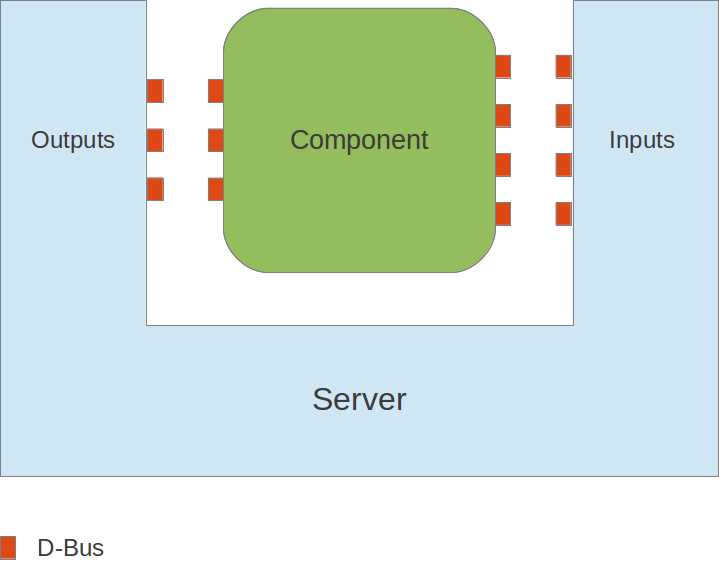
\includegraphics[width=0.6\columnwidth]{./figures/component.png}
\end{center}
\end{frame}

\begin{frame}{Components}
Code review
\end{frame}

\begin{frame}{Clients}
\textbf{Client can access to serveur with an API REST and an OAuth2 authentification.}
\vfill
\begin{columns}
\begin{column}[l]{0.5\textwidth}
\textbf{Web Interface :}
\vfill
\begin{figure}
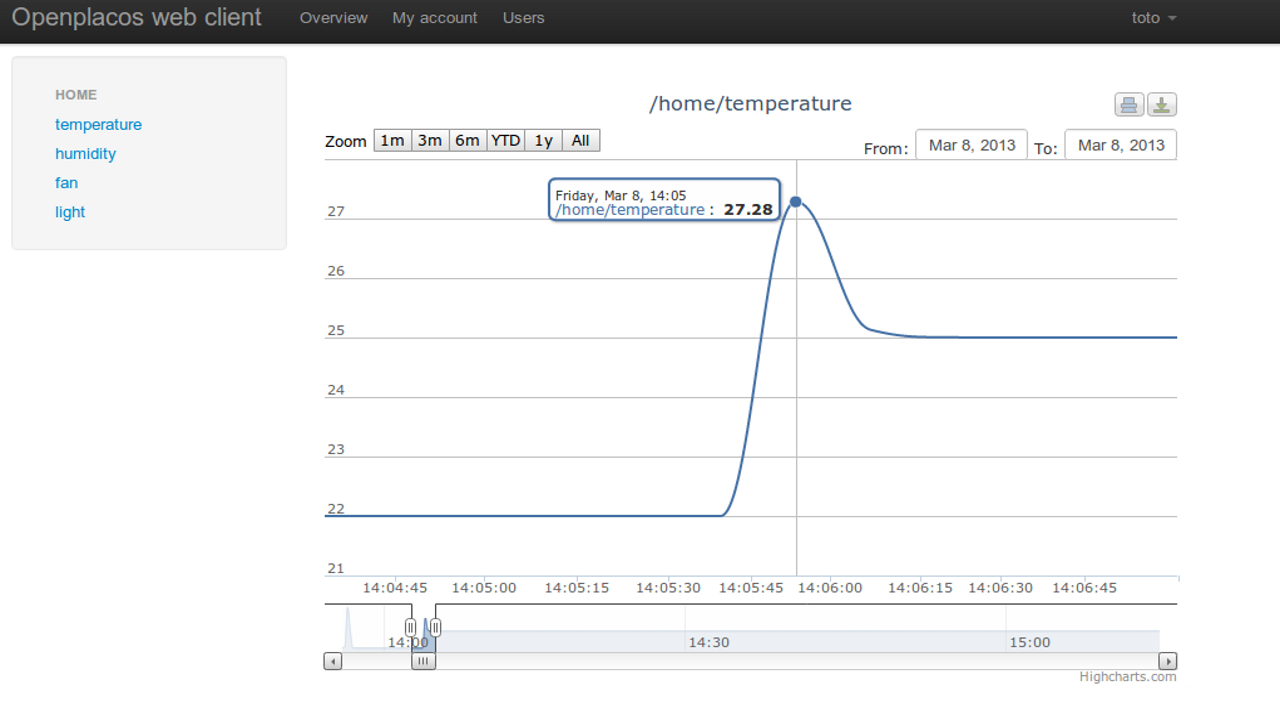
\includegraphics[width=\columnwidth]{./figures/oposweb.png}
\end{figure}
\end{column}
\begin{column}[r]{0.5\textwidth}
\textbf{Command Line :}
\vfill
\begin{figure}
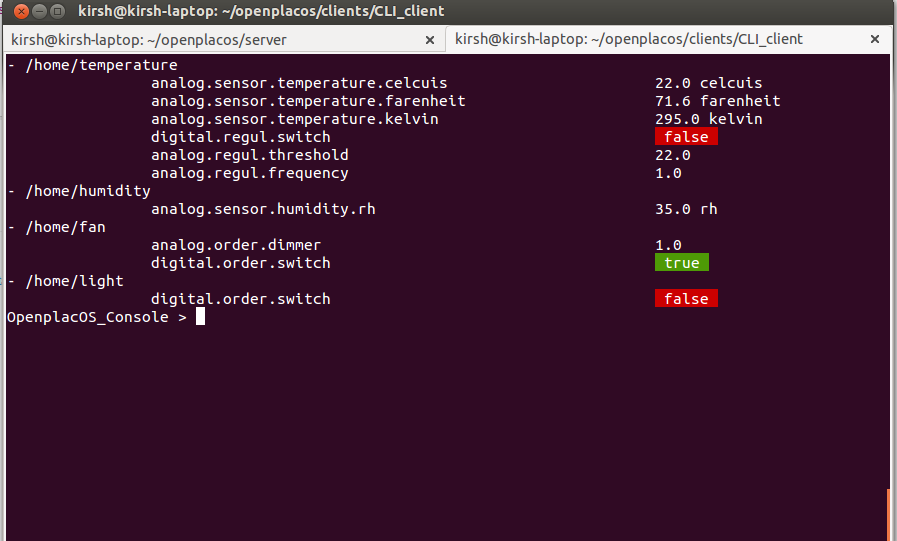
\includegraphics[width=\columnwidth]{./figures/oposcli.png}
\end{figure}
\end{column}
\end{columns}

\end{frame}

\begin{frame}{Core server}


\begin{figure}
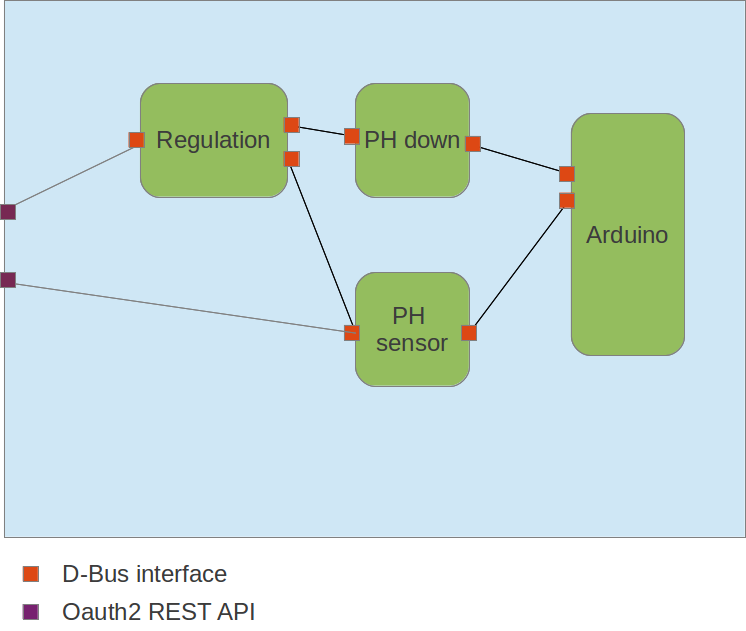
\includegraphics[width=0.7\columnwidth]{./figures/application.png}
\end{figure}
Core Server binds all components and expose them to a REST API.
\end{frame}
\section{Demo}

\begin{frame}{Demo1}
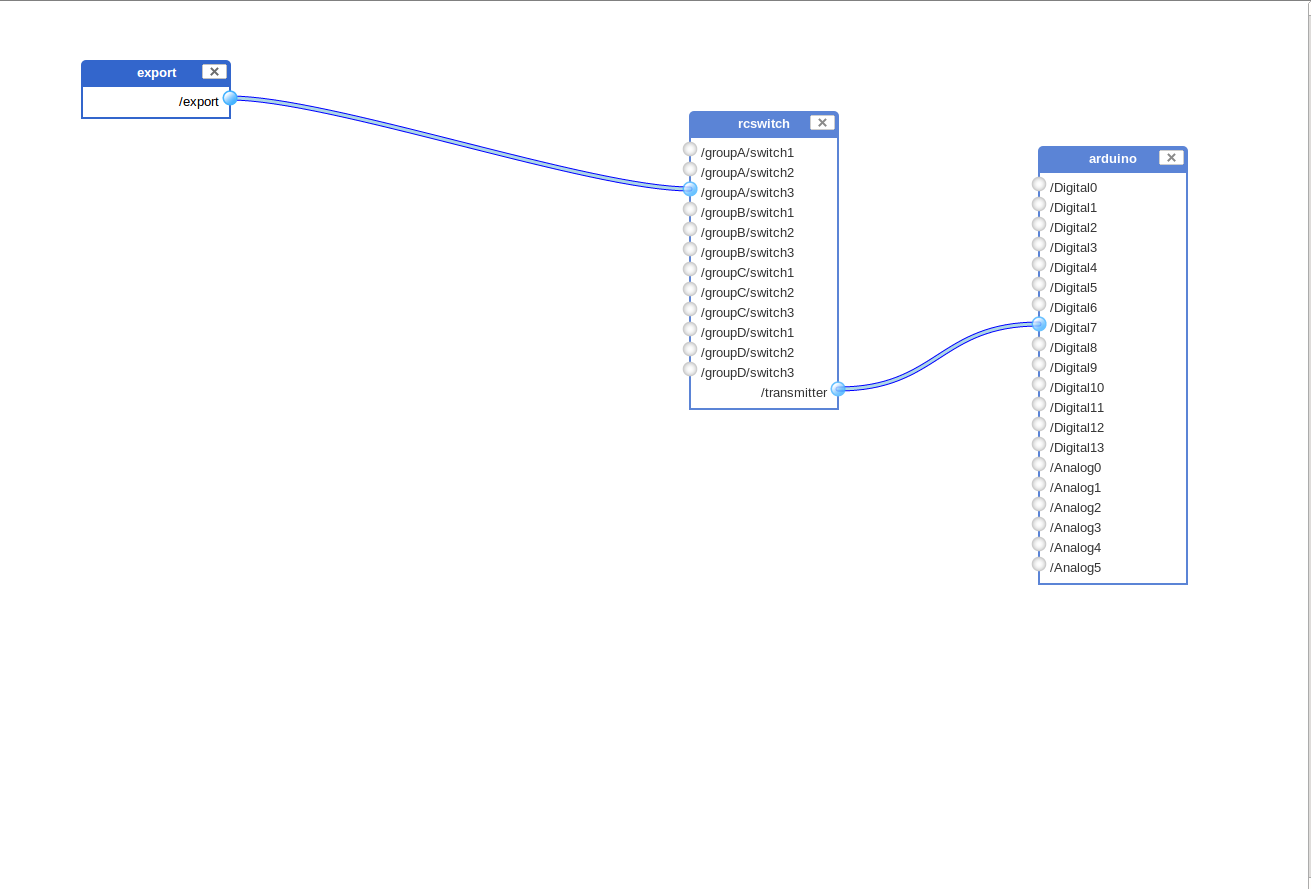
\includegraphics[width=\columnwidth]{figures/config1.png}
\end{frame}

\begin{frame}{Demo2}
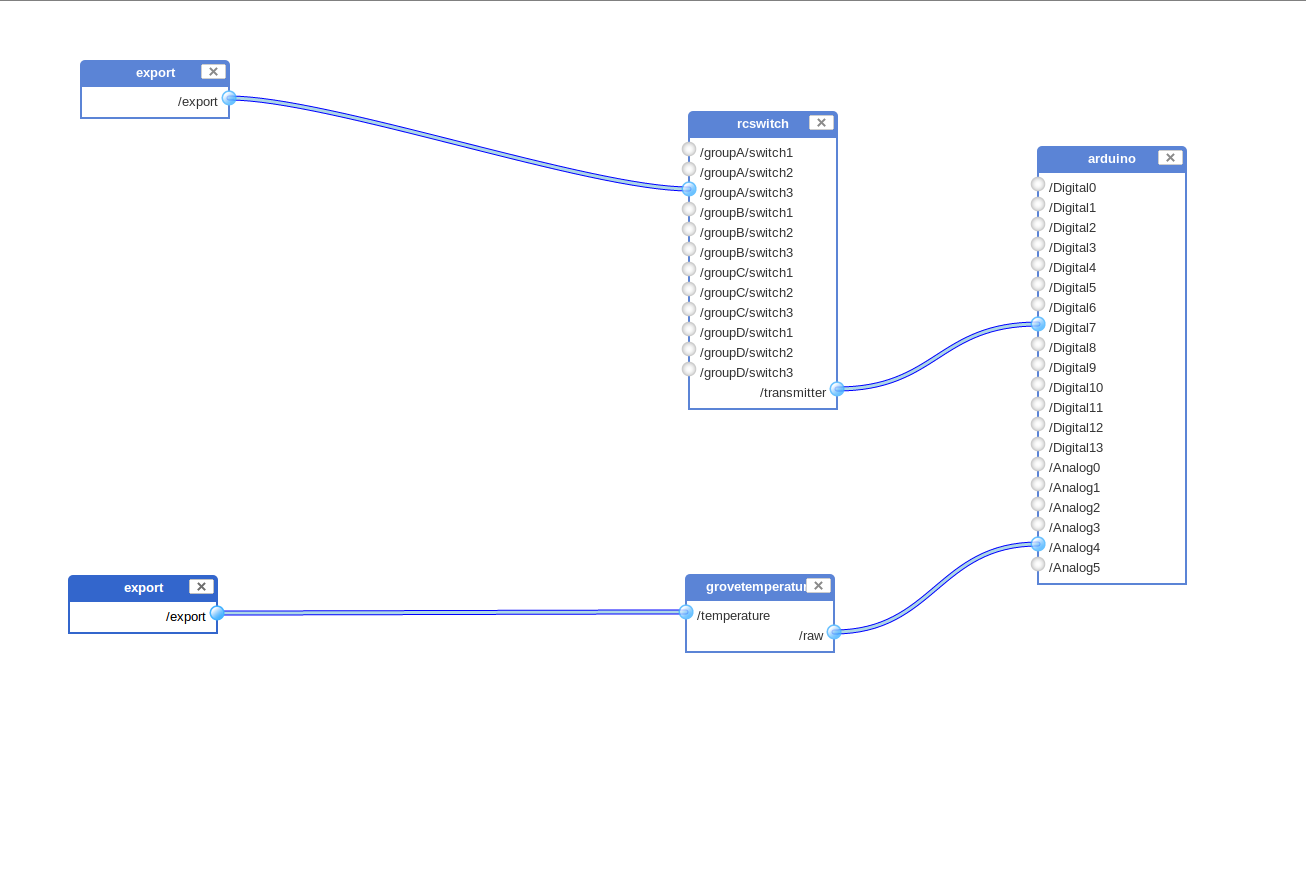
\includegraphics[width=\columnwidth]{figures/config2.png}
\end{frame}

\begin{frame}{Demo3}
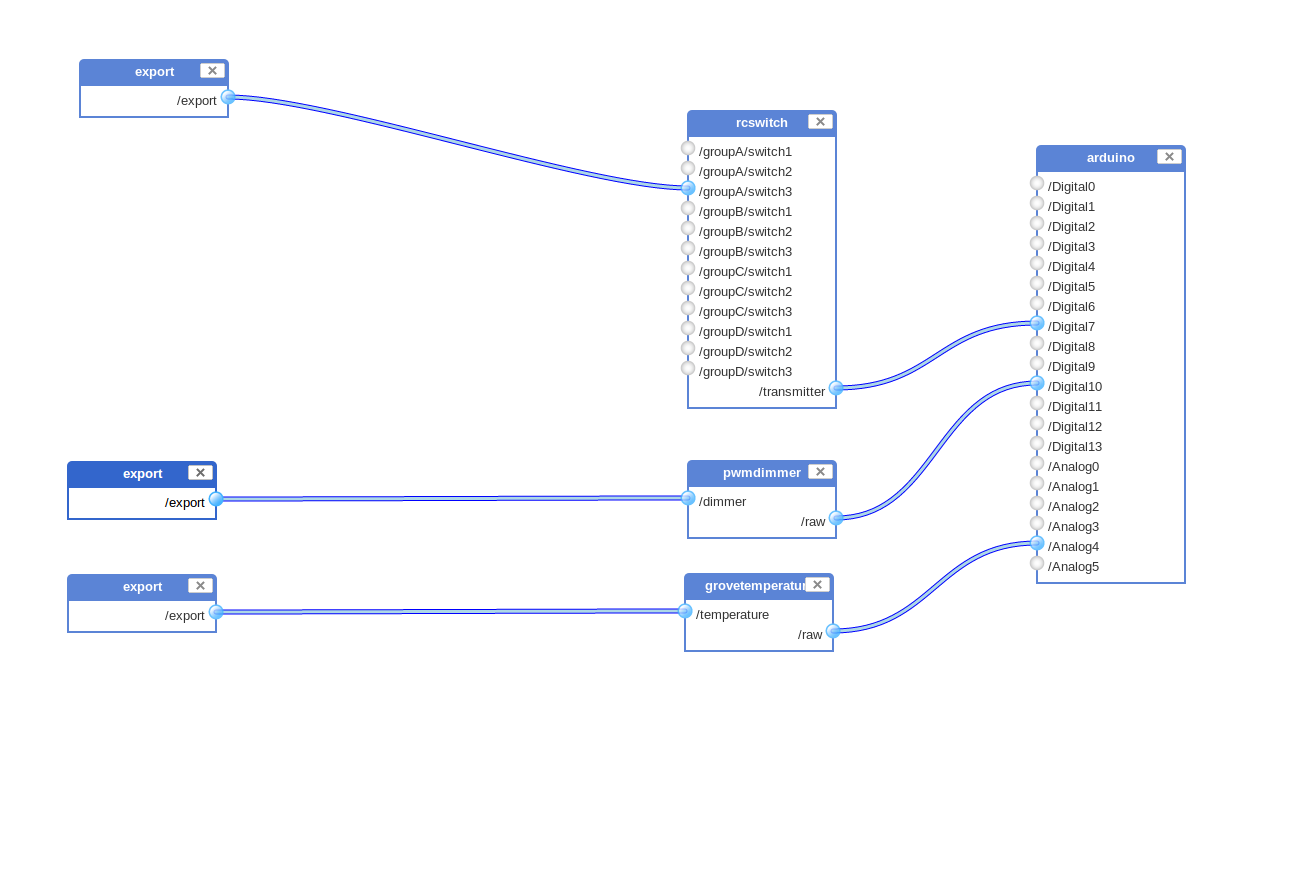
\includegraphics[width=\columnwidth]{figures/config3.png}
\end{frame}

\begin{frame}{Demo4}
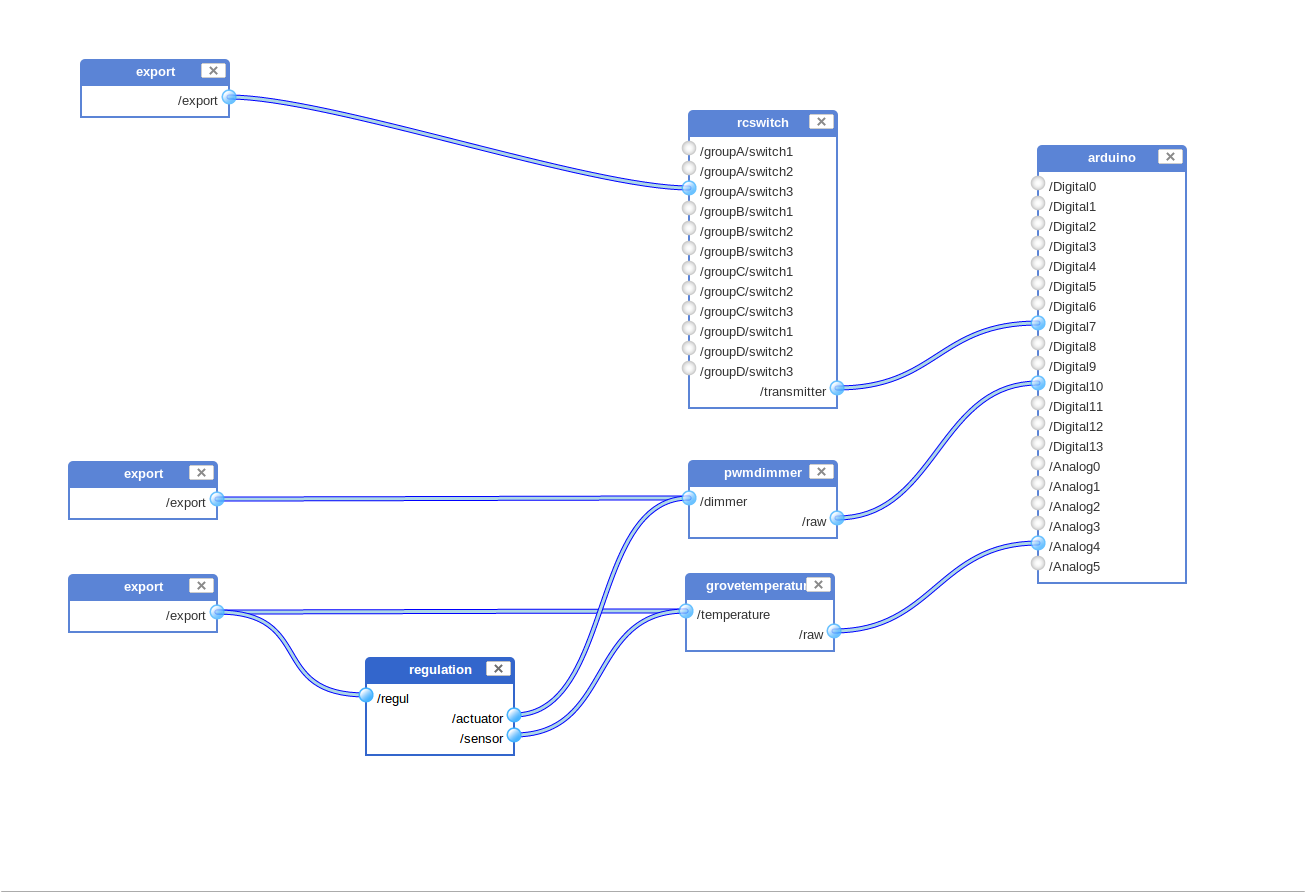
\includegraphics[width=\columnwidth]{figures/config4.png}

\end{frame}

\section{Conclusion}
\begin{frame}{Project status}
OpenplacOS is actually still in development:
 \begin{itemize}

\item Core server is functional and stable. Usable in daily life.
\item Still WIP in web interface and components library.
\item Packages avalaibles for ubuntu, debian, archlinux. 
\end{itemize}
\end{frame}
\begin{frame}{Perspectives}
2 active developments:
 \begin{itemize}
\item[$\Rightarrow$] Arduino shield for pH EC and temperature
\item[$\Rightarrow$] Graphical interface for config
\end{itemize}
\end{frame}
\end{document}
